% !TeX encoding = UTF-8
% !TeX program = pdflatex

\documentclass[11pt]{article}
\usepackage{graphicx}

\newcommand\CIPH{C\!I\!P\!H_K}

\title{{\bf The usage and the impact of shift registers on the CFB mode of operation} \\ \bigskip \large HW1 - CNS Sapienza}
\date{2018-10-12}
\author{Andrea Fioraldi 1692419}
\pagenumbering{roman}

\begin{document}
\maketitle

\section{Introduction}

With the aim to provide confidentiality and authenticity of information, {\em Block Ciphers} are widely used in cryptography. Block Ciphers operates on fixed-length messages, called {\em blocks}, and {\em Modes of Operations} are the techniques used to apply block ciphers to messages longer than a block.

{\em Cipher Feed Back} (CFB) is a popular mode of operation.
In the following sections, we will discuss the usage and the impact of CFB and, in particular, of its variant that uses shift registers.

\section{CFB Overview}

In this technique, regards the encryption, the produced cyphertext block is forwarded to the next encryption unit to produce a block of encrypted data that, xored\footnote{exclusive-ORed} with the correspondent plaintext block, generates the next ciphertext block. 

\begin{figure}[!ht]
  \centering
  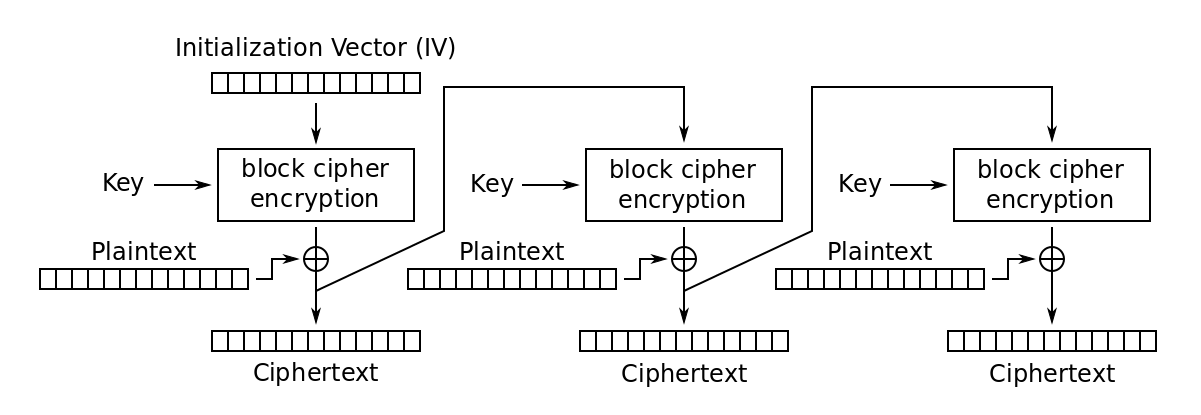
\includegraphics[width=1\textwidth]{pic1-hw1-1692419}
  \caption{CFB encryption, from \cite{wiki}}
  \label{fig:cfb_enc}
\end{figure}

Viceversa, during the decryption, the output of the encryption unit using the previous cyphertext block is xored with the current cyphertext block to produce the corresponding plaintext block.

\begin{figure}[!ht]
  \centering
  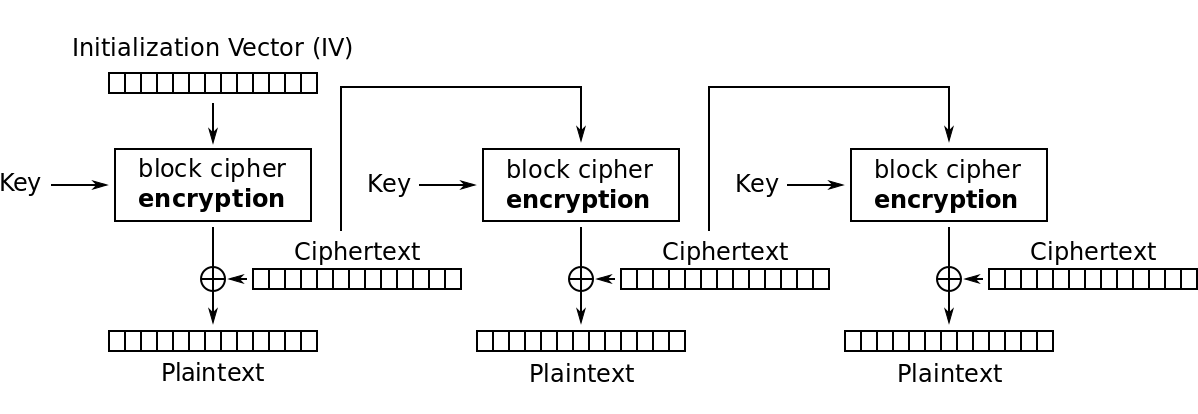
\includegraphics[width=1\textwidth]{pic2-hw1-1692419}
  \caption{CFB decryption, from \cite{wiki}}
  \label{fig:cfb_dec}
\end{figure}

This mode of operation requires an initialization vector (IV) as the initial input block. As you can see in figure \ref{fig:cfb_dec} the encryption unit is used also for decryption.

Accordingly to \cite{wiki}, CFB encryption and decryption can be expressed with the following formulas:

\begin{itemize}
\item Encryption: $C_0 = IV , C_i = \CIPH(C_{i-1}) \oplus P_i$;
\item Dencryption: $P_0 = IV , P_i = \CIPH(C_{i-1}) \oplus C_i$;
\end{itemize}

The used symbols are defined in the following way:

\begin{itemize}
\item $IV := $ the initialization vector;
\item $\CIPH := $ the encryption process using the key $K$;
\item $P_i := $ the i-th block of the plaintext;
\item $C_i := $ the i-th block of the cyphertext;
\end{itemize}

\section{CFB with Shift Registers}

One of the most used variants of CFB introduces shift registers as input for the encryption unit.

\subsection{Usage}

To describe the usage of shift registers in the CFB mode we must provide some additional definitions:

\begin{itemize}
\item $b := $ the size of a block in bits;
\item $s := $ the size of a plaintext/cyphertext segment in bits ($s \le b$);
\item $SR := $ the content of the input shift register;
\item $P_i := $ the i-th segment of the plaintext;
\item $C_i := $ the i-th segment of the cyphertext;
\end{itemize}

We define a {\em segment} as a block of the plaintext/cyphertext on which CFB operates. It can be smaller than the type of blocks used by $\CIPH$, so we use the term segment to distinguish between them.



\begin{figure}[!ht]
  \centering
  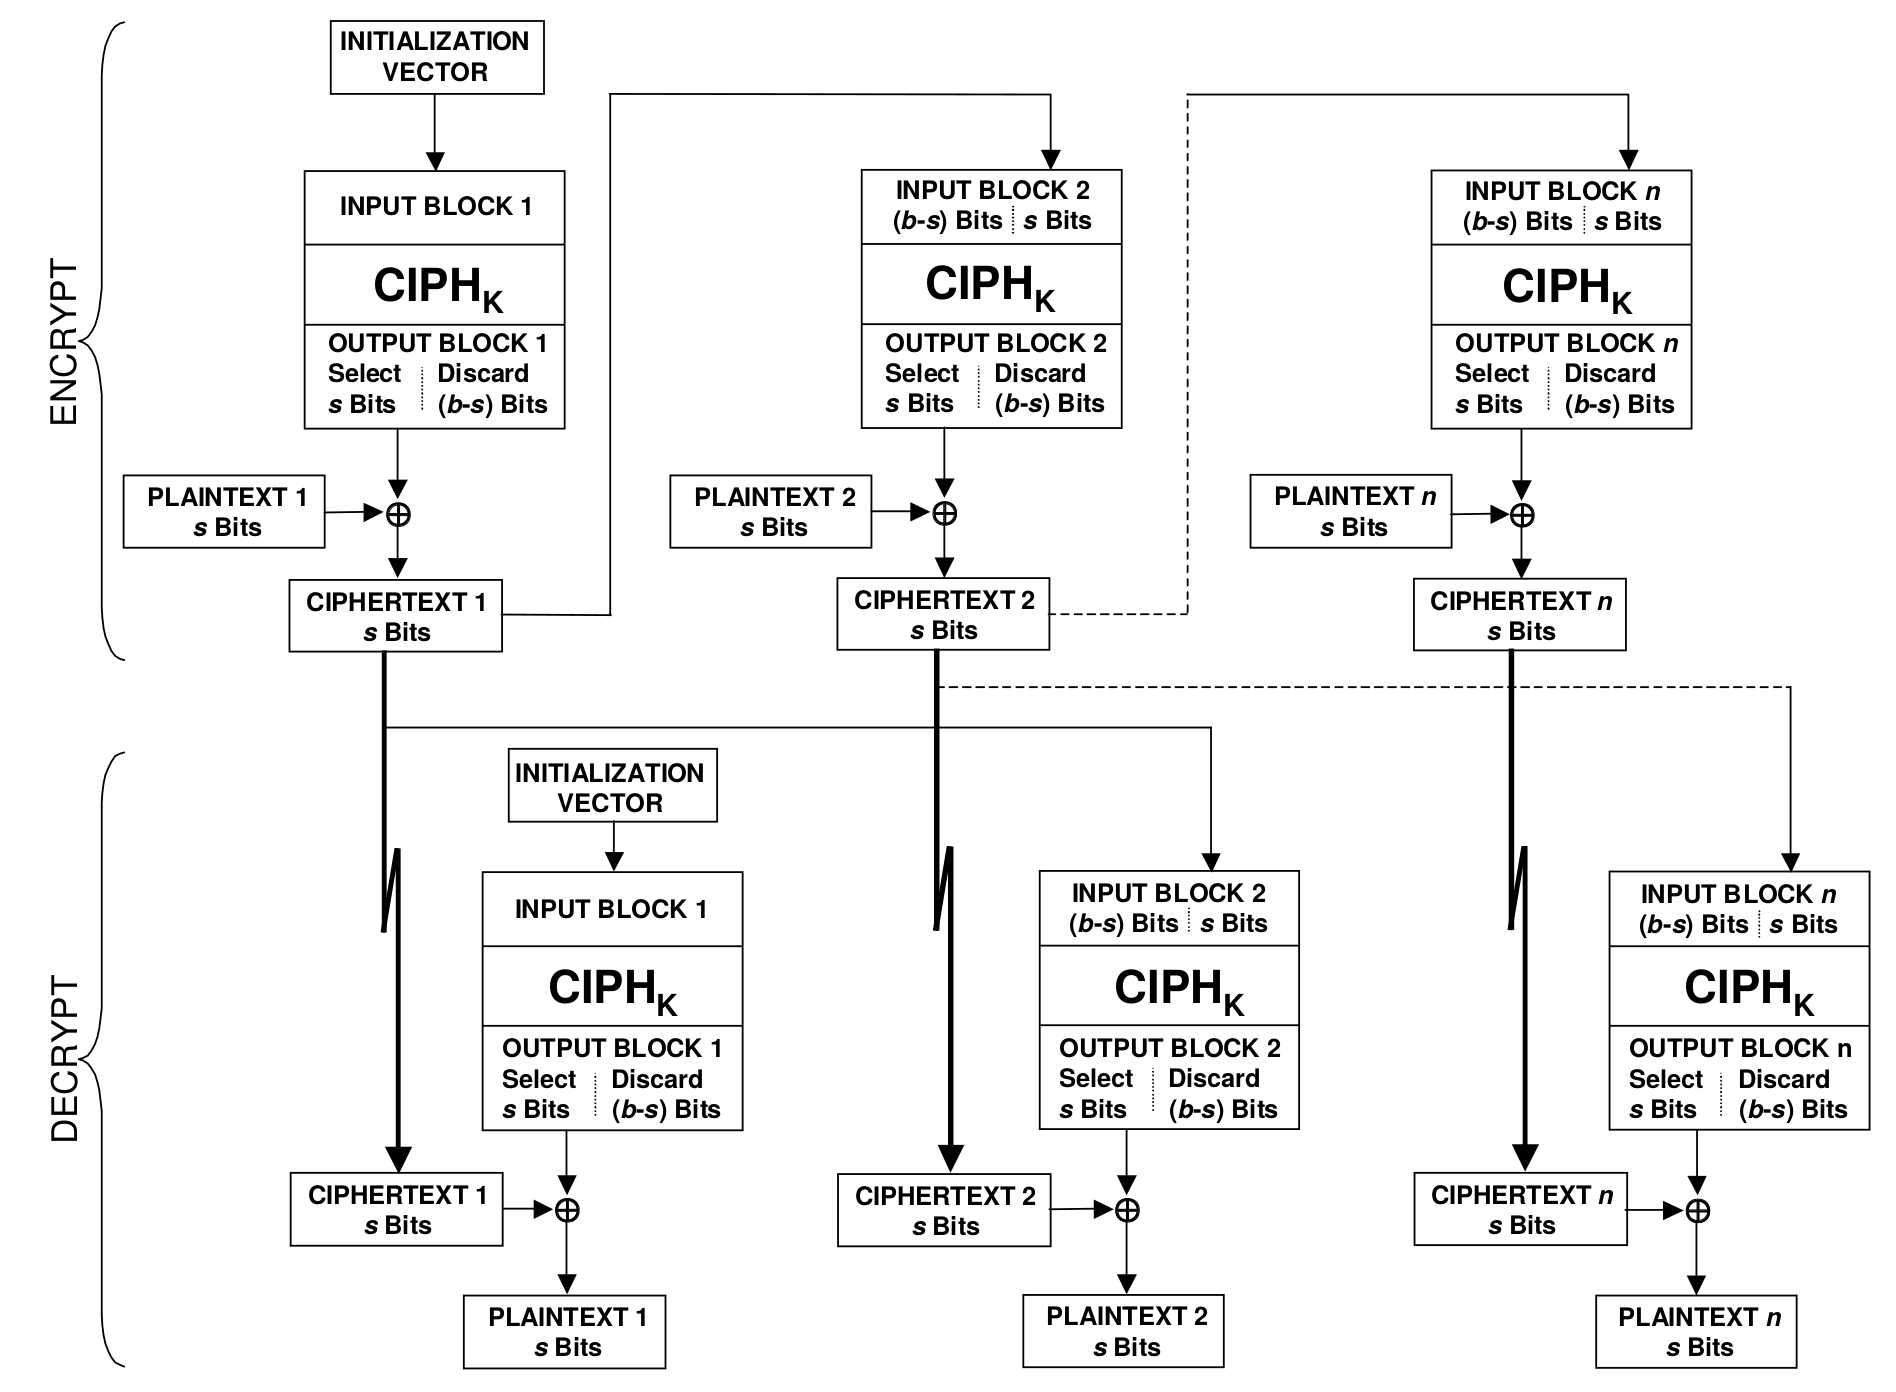
\includegraphics[width=1\textwidth]{pic3-hw1-1692419}
  \caption{CFB with shift registers, from \cite{nist}}
  \label{fig:cfb_shift}
\end{figure}

\subsection{Impact}



\newpage
\begin{thebibliography}{99}

\bibitem{wiki}
{\em Block cipher mode of operation - Wikipedia}.
  \verb|https://en.wikipedia.org/wiki/Block_cipher_mode_of_operation|
  \newblock Accessed: 2018-10-12.

\bibitem{nist}
Morris Dworkin.
  {\em Recommendation for Block Cipher Modes of Operation. Methods and Techniques}.
  Tech. rep. 800-38A. National Institute of Standards and Technology, 2001.
  \newblock \verb|url: http://www.dtic.mil/docs/citations/ADA400014|

\end{thebibliography}

\end{document}
